\documentclass[11pt,
  paper=a4, 
  bibliography=totocnumbered,
	captions=tableheading,
	BCOR=10mm
]{scrreprt}

\usepackage[utf8]{inputenc}
 
 
\usepackage[onehalfspacing]{setspace}
\usepackage{csquotes} % Context sensitive quotation.
\usepackage{amsmath} % Standard math.
\usepackage{amsthm} % Math theorems.
\usepackage{amssymb} % More math symbols.
\theoremstyle{definition}
\newtheorem{definition}{Definition}[chapter]
 
\usepackage[section]{placeins} % Keep floats in the section they were defined in.
\usepackage{tabularx}
\usepackage{booktabs} % Scientific table styling.
\usepackage{floatrow} % Option for keeping floats in the place they were defined in the code.
\floatsetup[table]{style=plaintop}
\usepackage{hyperref} % Hyperlinks.
\usepackage[all]{nowidow} % Prevent widows and orphans.
\usepackage{xstring} % logic string operations
\usepackage{bbm} % \mathbb on numerals.
\usepackage{csquotes}
\usepackage{mathtools}
\usepackage[ruled,vlined]{algorithm2e} % Pseudocode
\usepackage{scrhack} % Make warning go away.
\usepackage{graphicx}
\usepackage{subcaption} % Subfigures with subcaptions.
\usepackage{authoraftertitle} % Make author, etc., available after \maketitle
\usepackage{listofitems}
\usepackage{blindtext} % Placeholder text.
\usepackage[automake, nopostdot, nonumberlist]{glossaries} % glossary for definitions and acronyms, without dot after entry and page reference 
\makeglossaries % Generate the glossary

% \PassOptionsToPackage{obeyspaces}{url}%
\usepackage[backend=bibtex,% 
style=nature,% 
doi=true,isbn=false,url=false, eprint=false]{biblatex}
% \renewbibmacro*{url}{\printfield{urlraw}}

\addbibresource{references.bib}

\DeclareStyleSourcemap{
  \maps[datatype=bibtex, overwrite=true]{
    \map{
      \step[fieldsource=url, final]
      \step[typesource=misc, typetarget=online]
    }
    \map{
      \step[typesource=misc, typetarget=patent, final]
      \step[fieldsource=institution, final]
      \step[fieldset=holder, origfieldval]
    }
  }
}

%\linespread{1.5} % set line spacing
 
\usepackage{listings} % rendering program code
\lstset{% general command to set parameter(s)
	basicstyle=\ttfamily\color{grey},          % print whole listing small
	keywordstyle=\color{black}\bfseries\underbar,
	% underlined bold black keywords
	identifierstyle=,           % nothing happens
	commentstyle=\color{white}, % white comments
	stringstyle=\ttfamily,      % typewriter type for strings
	showstringspaces=false}     % no special string spaces


\DeclareFontFamily{U}{mathx}{\hyphenchar\font45}
\DeclareFontShape{U}{mathx}{m}{n}{
      <5> <6> <7> <8> <9> <10>
      <10.95> <12> <14.4> <17.28> <20.74> <24.88>
      mathx10
      }{}
\DeclareSymbolFont{mathx}{U}{mathx}{m}{n}
\DeclareFontSubstitution{U}{mathx}{m}{n}
\DeclareMathSymbol{\bigtimes}{1}{mathx}{"91}

 

%%% Custom definitions %%%
% Shorthands
\newcommand{\ie}{i.\,e.~}
\newcommand{\eg}{e.\,g.~}
\newcommand{\ind}{\mathbbm{1}}
% Functions
\newcommand{\tpow}[1]{\cdot 10^{#1}}
\newcommand{\figref}[1]{(Figure \ref{#1})}
\newcommand{\figureref}[1]{Figure \ref{#1}}
\newcommand{\tabref}[1]{(Table \ref{#1})}
\newcommand{\tableref}[1]{Table \ref{#1}}
\newcommand{\secref}[1]{%
	\IfBeginWith{#1}{chap:}{%
		(cf. Chapter \ref{#1})}%
		{(cf. Section \ref{#1})}%
		}
\newcommand{\sectionref}[1]{%
	\IfBeginWith{#1}{chap:}{%
		Chapter \ref{#1}}%
		{\IfBeginWith{#1}{s}{%
			Section \ref{#1}}%
			{[\PackageError{sectionref}{Undefined option to sectionref: #1}{}]}}}
\newcommand{\chapref}[1]{(see chapter \ref{#1})}
\newcommand{\unit}[1]{\,\mathrm{#1}}
\newcommand{\unitfrac}[2]{\,\mathrm{\frac{#1}{#2}}}
\newcommand{\codeil}[1]{\lstinline{#1}}{} % wrapper for preventing syntax highlight error
\newcommand{\techil}[1]{\texttt{#1}}
\newcommand{\Set}[2]{%
  \{\, #1 \mid #2 \, \}%
}
% Line for signature.
\newcommand{\namesigdate}[1][5cm]{%
	\vspace{5cm}
	{\setlength{\parindent}{0cm}
	\begin{minipage}{0.3\textwidth}
		\hrule 
		\vspace{0.5cm}
		{\small city, date}
	\end{minipage}
	 \hfill
	\begin{minipage}{0.3\textwidth}
		\hrule
		\vspace{0.5cm}
	    {\small signature}
	\end{minipage}
	}
}
% Automatically use the first sentence in a caption as the short caption.
\newcommand\slcaption[1]{\setsepchar{.}\readlist*\pdots{#1}\caption[{\pdots[1].}]{#1}}

% Variables. 
% Adapt if necessary, use to refer to figures and graphics.
\def \figwidth {0.9\linewidth}
\graphicspath{ {./graphics/figures/}{./graphics/figures/} } % Path to figures and images.


% Customizations of existing commands.
\renewcommand{\vec}[1]{\mathbf{#1}}
% Capitalized \autoref names.
\renewcommand*{\chapterautorefname}{Chapter}
\renewcommand*{\sectionautorefname}{Section}


% TODO Fill with your data.
\title{My full title}
\author{Christoph Stenkamp}

\begin{document}

\begin{titlepage}
	\begin{flushleft}
		Universität Osnabrück\\
		Fachbereich Humanwissenschaften\\
		Institute of Cognitive Science
	\end{flushleft}

	\vspace{2cm}
	\centering{
		Master's thesis\vspace{1cm}\\
		\textbf{\Large{\MyTitle}}
		\vspace{1cm}\\
		\begin{tabular}{c}
			\MyAuthor                          \\
			955004                             \\
			Master's Program Cognitive Science \\
			April 2017 - Dezember 2021
		\end{tabular}}
	\vspace{1cm}

	\begin{tabular}{ll}
		First supervisor:  & Dr. Tobias Thelen          \\
		                   & Institute of Cognitive Science \\
		                   & University of Osnabrück  \\\\
		Second supervisor: & Prof. Dr. Someone Else         \\
		                   & Institute of Cognitive Science \\
		                   & Osnabrück
	\end{tabular}

\end{titlepage}


\chapter*{Declaration of Authorship}
I hereby certify that the work presented here is, to the best of my knowledge and belief, original and the result of my own investigations, except as acknowledged, and has not been submitted, either in part or whole, for a degree at this or any other university.

\namesigdate
\pagenumbering{gobble}
\pagebreak

\begin{abstract}
	\textbf{\LARGE{Abstract}}\\\\
	%TODO summarize the main objectives and outcomes of your work. The abstract should fit on one page.
	In this thesis, I want to generate a conceptual space for the domain of university courses, automatically created in data-driven way from their descriptions.
\end{abstract}




\tableofcontents
\listoffigures
\listoftables
\listofalgorithms


\chapter{Introduction}
\pagenumbering{arabic}

In this thesis, I want to generate a conceptual space for the domain of university courses, automatically created in data-driven way from their descriptions.

\section{What are conceptual spaces? }

Conceptual spaces (Gärdenfors, blabla) want to stand in between subsymbolic processing and symbolic processing: Like in subsymbolism, concepts are represented in high-dimensional spaces, but because the dimensions of these spaces are not arbitrary but human-interpretable, it allows for symbolistic high-level reasoning.

So, in conceptual spaces, concepts are represented as convex regions in high-dimensional, human interpretable spaces. For example, the concept of "apple" is a region that in the dimension "color" is somewhere between red and green, in the dimension "form" at roughly round, in the dimension "taste" somwhere between sweet and sour, etc. 
Every instance of an apple is thus a vector that lies inside the high-dimensional region of the concept. This allows for high-level reasoning, such as the question "does concept X fit into my bag?" -> If the "size" dimension of the size is smaller than the size of my bag, it will.

Conceptual spaces sounds similar to word2vec or other word embedding approaches, however there are a few important distinctions - first, the domain of a conceptual space does not include all kinds of words or concepts, but only concepts of a certain domain (like movies or university courses). 
Second, conceptual spaces are convex regions, not mere vectors (which allows for easy extraction of is-a and part-of relations or prototypical examples vs edge examples, but makes the generation computationally vastly more expensive). And, most importantly, while the geometry of word2vec is roughly euclidian (otherwise the famous vec(king)-vec(man)+vec(woman)==vec(queen) wouldn't work), the dimensions are not interpretable but arbitrarily depend on the random initial setup, so the concepts king and queen differ not only in a single "gender" dimension [..and also its not really euclidian, is it?! sonst wäre die betweeness doch nicht so special, oder?].

Now the standard problem with conceptual spaces is that they would have to be manually generated, which of courses is a lot of work, which is where the work of [Schokeart et al] comes in - to generate them in a data-driven fashion.
For that, the authors look at three different domains: movies, wines and places. For each of these domains, they collected many samples (like movies) together with descriptions from places where people can leave them (like reviews from IMDB). A representation of a movie is then generated from the bag-of-words of the descriptions of the individual movies, leading to a very high-dimensional, very sparse representation for all movies. 
To make the representations less sparse and more meaningful, the words in the BOW are subsequently PPMI-weighted, which weights words that appear often in the description of a particular movie while being infrequent in the corpus overall higher while setting the representation of stopwords to almost zero. 
This PPMI-weighted BOW is however not yet a euclidian space yet, which is why the authors subsequently use multidimensional scaling (MDS). MDS is a diminsionality reduction technique that attempts to create a euclidian space of lower dimensionality than the original one in which the individual distances of the items are preserved as well as possible. 

With such a space, the concepts of betweeness already makes sense, but so far, the dimensions are not interpretable. So how does one automatically find such directions? In the case of movies, good dimensions may be "scariness", "funniness", "epicness", "family-friendlyness" etc. 
To find these dimensions, the authors look for these words (as well as similar words thanks to clustering) in the reviews. Then the movies are grouped into those that contain the words from the cluster often enough vs those that don't. A support-vector-machine subsquently finds a hyperplane that best divides the two groups (eg. scary and non-scary), and the orthogonal of that hyperplane is used as one axis of the new coordinate basis. 

% TODO: Ist word2vec schon nen euclidian space? Why/Why not?

% \begin{figure}[H]
% 	\centering
% 	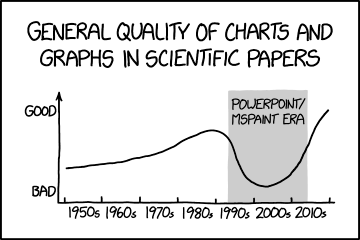
\includegraphics[width=\figwidth]{scientific_paper_graph_quality}
% 	\slcaption{
% 		Developmemt of scientific paper graph quality. A dip in the
% 		quality of scientific graphs is observed from the early 1990s to the early 2010s.
% 		During this time Microsoft Paint and PowerPoint were often used to create graphs in scientific papers.\label{fig:scientific_graph_quality}}
% \end{figure}

% \begin{table}[H]
% 	\begin{tabular}{@{}ll@{}}
% 		\toprule
% 		year & quality \\ \midrule
% 		1985 & good    \\
% 		2000 & bad     \\ \midrule
% 		2015 & better  \\ \bottomrule
% 	\end{tabular}
% 	\caption{
% 		Empirical measurements of scientific graph quality. Data points were collected using
% 		a systematic literature review.\label{tab:scientific_graph_quality}}
% \end{table}
% This references a \figref{fig:scientific_graph_quality} while this references a table \tabref{tab:scientific_graph_quality}.

% A citation looks like this \cite{hadash2018estimate}. To embed a citation in the text flow use textcite,
% \eg \textcite{hadash2018estimate} said you should use a lot of citations.

\chapter{Methods}


\chapter{Results and Discussion}


\chapter{Conclusion}


\chapter*{Acknowledgements}
%TODO A place to say thank you to everybody who helped you.


% START Acronym definitions
\newacronym{utc}{UTC}{Universal Time Coordinated}
\newacronym{ml}{ML}{Machine Learning}
% END Acronym definitions

\glsaddall
\printglossaries

\printbibliography

\end{document}
